\lstset{language=VBScript,
        basicstyle=\footnotesize\ttfamily,
        breaklines=true,
        tabsize=2,
        numbers=left,
        numberstyle=\tiny,
        numbersep=7pt,
        showspaces=false,
        keywordstyle=\color{Blue}\textbf,
        commentstyle=\color{Red}\emph,
        showstringspaces=false,
        stringstyle=\color{BurntOrange}
        }
\section{Instrukcja użytkownika}
%\subsection{Specyfikacja zewnętrzna}
Zaimplementowana przez autora wizualizacja ma na~celu zobrazowanie działania modelu oraz umożliwienie operatorowi wpływania na~jego działanie. Kolejne podrozdziały zawierają opis specyfikacji zewnętrznej oraz wewnętrznej. Część odnosząca się do specyfikacji zewnętrznej jest skróconą instrukcją obsługi użytkownika. Specyfikacja wewnętrzna jest opisem, jak zostały zrealizowane poszczególne elementy~i~w jaki sposób wizualizacja współpracuje ze~sterownikiem.

Ekrany dostępne w wizualizacji oraz klawisze funkcyjne z nimi związane:
\begin{itemize} 
\item Ekran powitalny - F1,
\item Stan robota - F2,
\item Stan magazynu i testowanie obsługi - F3,
\item Testowanie sterowania ręcznego z pilota podłączonego do sterownika - F4,
\item Testowanie sterowania ręcznego z poziomu wizualizacji - F5,
\item Testowanie sterowania automatycznego - F6.
\end{itemize}
\indent
\indent Poszczególne ekrany zostaną szczegółowo opisane w kolejnych podrozdziałach.

\begin{figure}[!htb] 	\centering 	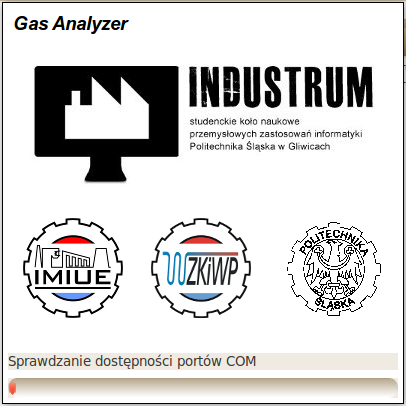
\includegraphics[width=0.5\textwidth]{images/splashScreen.png} \caption{Okno ładowania} \label{template} \end{figure}

\subsubsection{Ekran powitalny}
Bezpośrednio po~uruchomieniu wizualizacji użytkownik zobaczy ekran powitalny taki jak na Rysunku~\ref{main} zawierający informacje o~autorze projektu, osobie kierującej projektem (promotorze) oraz informację o~przeznaczeniu wizualizacji wraz ze~zdjęciem modelu. Dodatkowo na~ekranie tym umieszczony został zegar analogowy i~cyfrowy oraz aktualna data.
\begin{figure}[!htb]
\centering 		
  \subfloat[Windows]{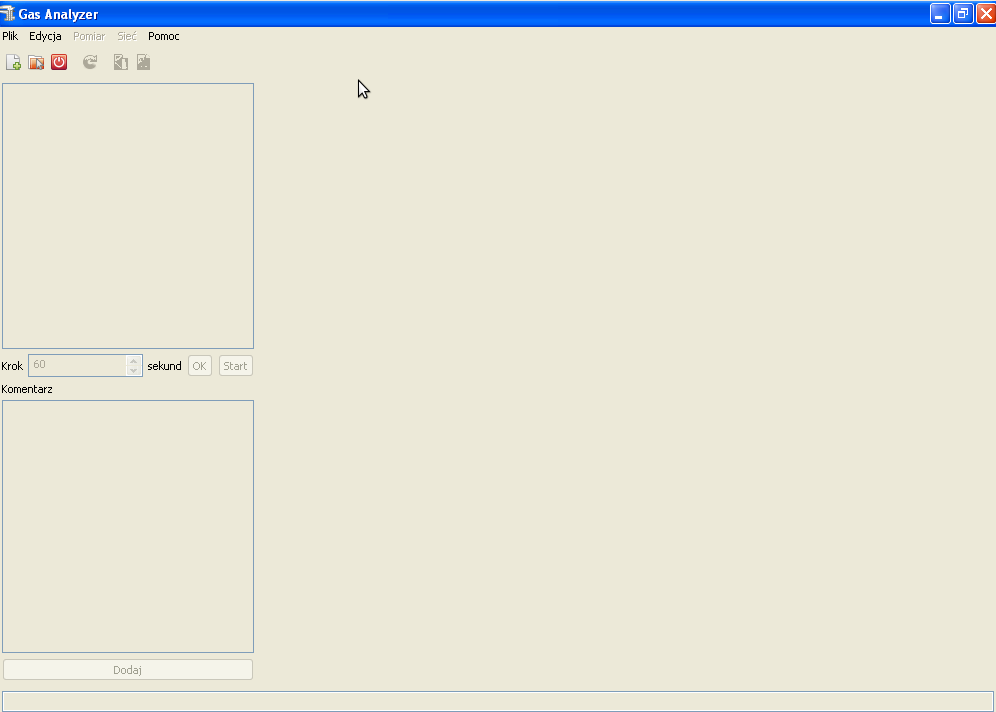
\includegraphics[width=0.45\textwidth]{images/mainW}}   
  \hspace{2mm}          
  \subfloat[Linux]{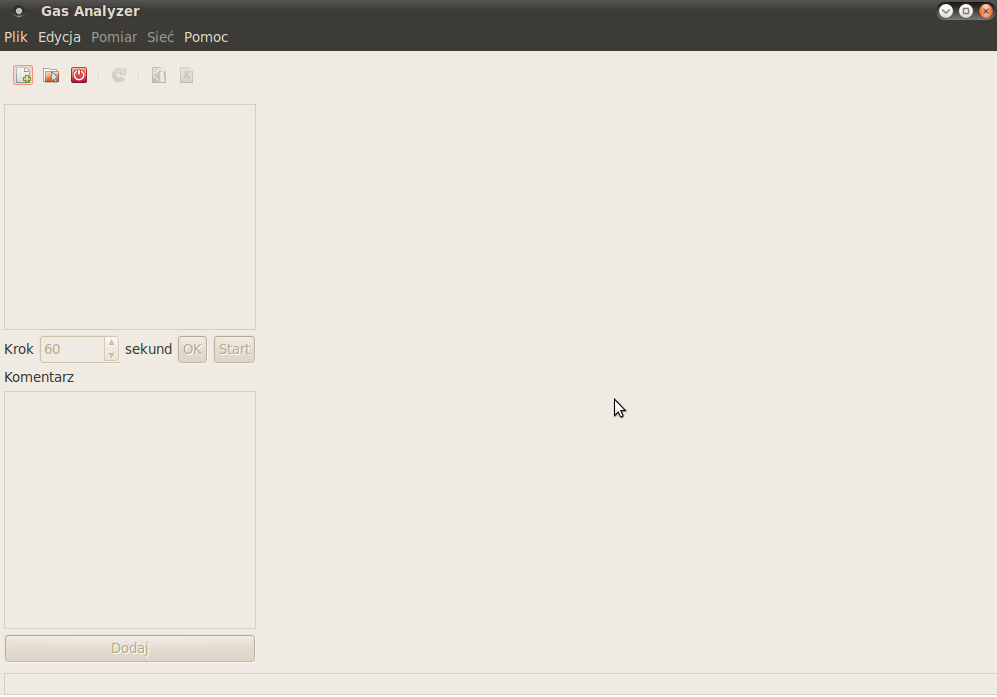
\includegraphics[width=0.45\textwidth]{images/mainL}}
\caption{Okno główne} 	
\label{main}
\end{figure}

\begin{figure}[!htb]
\centering 		
  \subfloat[Windows]{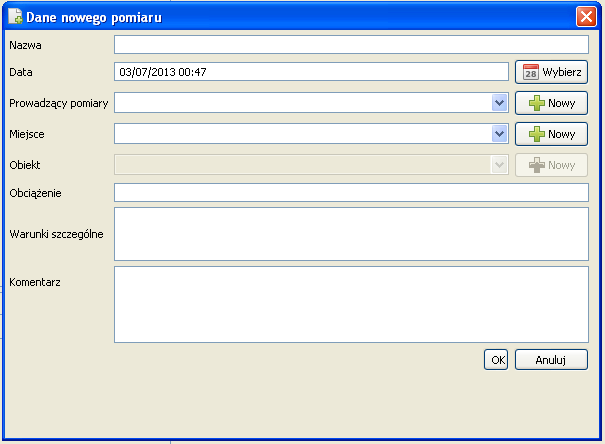
\includegraphics[width=0.45\textwidth]{images/newSurveyW}}                
  \hspace{2mm}
  \subfloat[Linux]{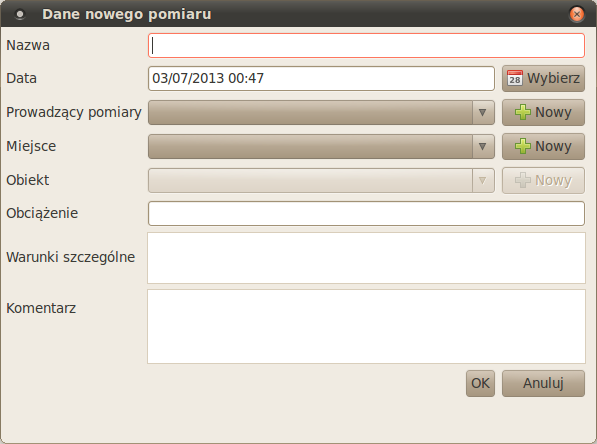
\includegraphics[width=0.45\textwidth]{images/newSurveyL}}
\caption{Dodawanie nowego pomiaru} 	
\label{main}
\end{figure}

\begin{figure}[!htb]
\centering 		
  \subfloat[Windows]{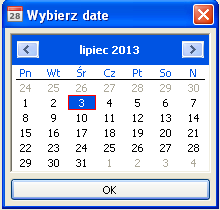
\includegraphics[width=0.25\textwidth]{images/calendarW}}    
  \hspace{2mm}
  \subfloat[Linux]{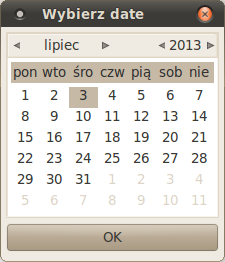
\includegraphics[width=0.25\textwidth]{images/calendarL}}
\caption{Okno wyboru daty} 	
\label{main}
\end{figure}

\begin{figure}[!htb]
\centering 		
  \subfloat[Windows]{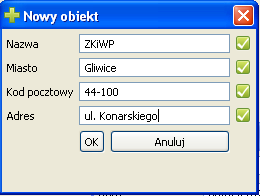
\includegraphics[width=0.45\textwidth]{images/newPlaceW}}                
  \hspace{2mm}
  \subfloat[Linux]{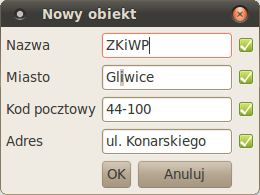
\includegraphics[width=0.45\textwidth]{images/newPlaceL}}
\caption{Dodawanie nowego miejsca} 	
\label{main}
\end{figure}

\begin{figure}[!htb]
\centering 		
  \subfloat[Windows]{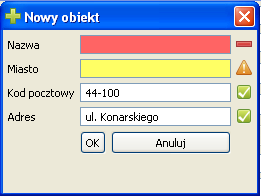
\includegraphics[width=0.45\textwidth]{images/newPlaceErrorW}}                
  \hspace{2mm}
  \subfloat[Linux]{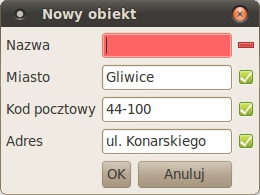
\includegraphics[width=0.45\textwidth]{images/newPlaceErrorL}}
\caption{Błąd przy dodawaniu nowego miejsca} 	
\label{main}
\end{figure}

\begin{figure}[!htb]
\centering 		
  \subfloat[Windows]{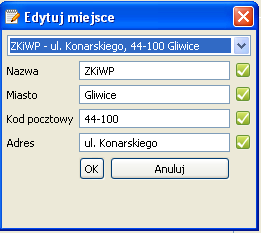
\includegraphics[width=0.45\textwidth]{images/editPlaceW}}                
  \hspace{2mm}
  \subfloat[Linux]{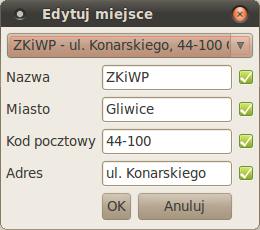
\includegraphics[width=0.45\textwidth]{images/editPlaceL}}
\caption{Edytowanie istniejącego miejsca} 	
\label{main}
\end{figure}

\begin{figure}[!htb]
\centering 		
  \subfloat[Windows]{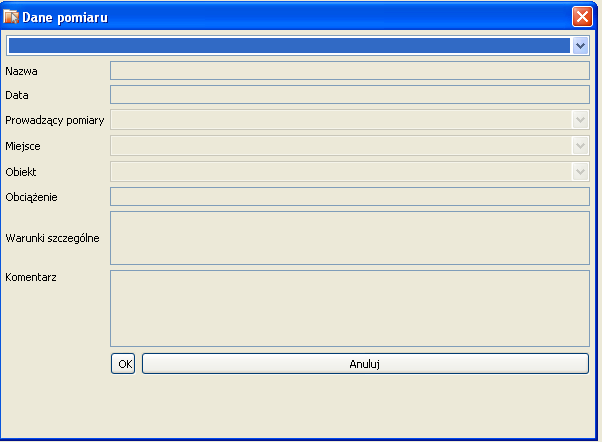
\includegraphics[width=0.45\textwidth]{images/openSurveyW}}                
  \hspace{2mm}
  \subfloat[Linux]{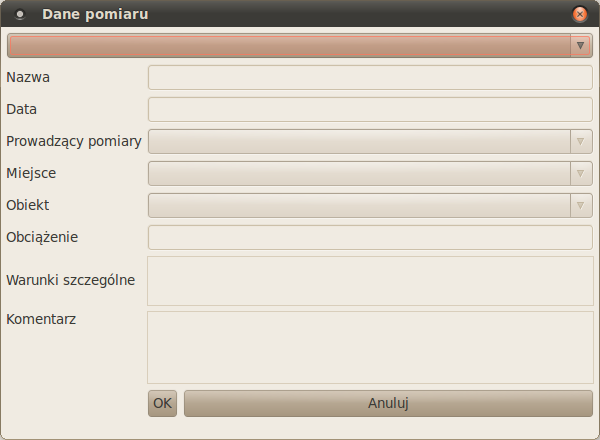
\includegraphics[width=0.45\textwidth]{images/openSurveyL}}
\caption{Otwieranie istniejącego pomiaru} 	
\label{main}
\end{figure}

\begin{figure}[!htb]
\centering 		
  \subfloat[Windows]{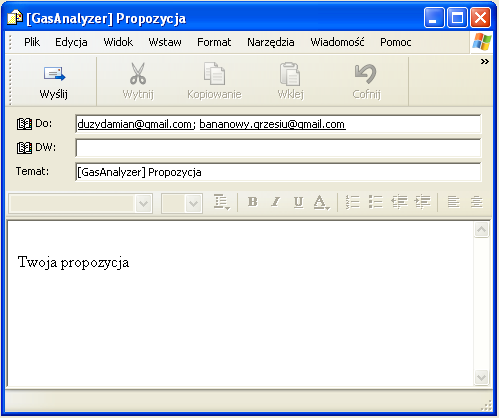
\includegraphics[width=0.45\textwidth]{images/suggestionW}}                
  \hspace{2mm}
  \subfloat[Linux]{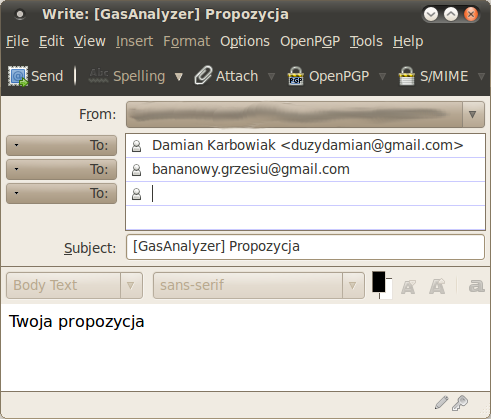
\includegraphics[width=0.45\textwidth]{images/suggestionL}}
\caption{Wysyłanie sugestii} 	
\label{main}
\end{figure}